% !TeX root = ../paper.tex
\section{Numerical experiments}\label{sec:DR_experiments}


\begin{figure}
    \centering
    \includegraphics[width=\linewidth]{figures/SNEkhorn/heteroscedastic_noise.pdf}    \caption{From left to right: entries of $\overline{\Pb^{\mathrm{e}}}$ \eqref{symmetrization_tsne} and associated embeddings generated using $\overline{\Pb^{\mathrm{e}}}$. Then $\Pb^{\mathrm{se}}$ \eqref{eq:sym_entropic_affinity} matrix and associated SNEkhorn embeddings. Perplexity $\xi = 30$.}
    \label{fig:simulated_data_multinomial}
\end{figure}

This section aims at illustrating the performances of the proposed affinity
matrix $\Pb^{\mathrm{se}}$ \eqref{eq:sym_entropic_affinity} and DR method SNEkhorn at faithfully representing dependencies and
clusters in low dimensions. First, we showcase the relevance of our approach on a simple synthetic dataset with heteroscedastic noise. 
% (Section
% \ref{sec:simulated_data}). 
Then, we evaluate the spectral clustering
performances of symmetric entropic affinities before benchmarking
t-SNEkhorn with t-SNE and UMAP \cite{mcinnes2018umap} on real-world images and genomics datasets.
% (Section \ref{sec:exp_real_data}).

% \subsection{Simulated data}\label{sec:simulated_data}
% \begin{minipage}{0.48\linewidth} 
% \textbf{Simulated data.}
% We take inspiration from \cite{landa2021doubly} and consider the task of discriminating between samples from two multinomial distributions. We first sample uniformly two vectors $\p_1$ and $\p_2$ in the $10^4$-dimensional probability simplex. We then generate $n=10^3$ samples as $\x_i =\tilde{\x}_i / (\sum_j \tilde{x}_{ij})$ such that:
% \begin{align*}
%     \tilde{\x}_i \sim 
%     \left\{
%     \begin{array}{ll}
%         \mathcal{M}(10^3, \p_1), & 1\leq i \leq 500 \\
%         \mathcal{M}(10^3, \p_2), & 501\leq i \leq 750 \\
%         \mathcal{M}(10^4, \p_2), & 751\leq i \leq 1000 \:.
%     \end{array}
%     \right.
% \end{align*}
% where $\mathcal{M}$ stands for the multinomial distribution. 
% The goal of the task is to test the robustness to heteroscedastic noise. Indeed, points generated using $\p_2$ exhibit different levels of noise due to various numbers of multinomial trials ($10^3$ and $10^4$) to form an estimation of $\p_2$. This typically occurs in real-world scenarios when the same entity is measured using different experimental setups thus creating heterogeneous technical noise levels (\eg in single-cell sequencing \cite{kobak2019art}). This phenomenon is known as \emph{batch effect} \cite{tran2020benchmark}.
% \end{minipage}
% \hspace{0.005\linewidth}
% \begin{minipage}{0.5\linewidth}
% \vspace{-1mm}
% \centering
% \includegraphics[width=\linewidth]{figures/heteroscedastic_noise.pdf}
%  \captionof{figure}{Top: entries of $\overline{\Pb^{\mathrm{e}}}$ \eqref{symmetrization_tsne} and $\Pb^{\mathrm{se}}$ \eqref{eq:sym_entropic_affinity} matrices. Bottom: embeddings generated by symmetric-SNE and SNEkhorn using the above affinities. Perplexity $\xi = 30$.}
% \label{fig:simulated_data_multinomial}
% \end{minipage}

\textbf{Simulated data.}
We take inspiration from \cite{landa2021doubly} and consider the task of discriminating between samples from two multinomial distributions. We first sample uniformly two vectors $\pb_1$ and $\pb_2$ in the $10^4$-dimensional probability simplex. We then generate $n=10^3$ samples as $\xb_i =\tilde{\xb}_i / (\sum_j \tilde{x}_{ij})$ such that:
\begin{align*}
    \tilde{\xb}_i \sim 
    \left\{
    \begin{array}{ll}
        \mathcal{M}(10^3, \pb_1), & 1\leq i \leq 500 \\
        \mathcal{M}(10^3, \pb_2), & 501\leq i \leq 750 \\
        \mathcal{M}(10^4, \pb_2), & 751\leq i \leq 1000 \:.
    \end{array}
    \right.
\end{align*}
where $\mathcal{M}$ stands for the multinomial distribution. 
The goal of the task is to test the robustness to heteroscedastic noise. Indeed, points generated using $\mathbf{p}_2$ exhibit different levels of noise due to various numbers of multinomial trials ($10^3$ and $10^4$) to form an estimation of $\mathbf{p}_2$. This typically occurs in real-world scenarios when the same entity is measured using different experimental setups thus creating heterogeneous technical noise levels (\eg in single-cell sequencing \cite{kobak2019art}). This phenomenon is known as \emph{batch effect} \cite{tran2020benchmark}.
% In single-cell sequencing, $\p_1$ and $\p_2$ can represent the probability of expressing genes in two different cells (these data are prone to suffer from high variability in technical noise.)
% As suspected in \cite{landa2021doubly}, the usual stochastic affinity used in t-SNE performs poorly when there is variability in the noise level.
In \cref{fig:simulated_data_multinomial}, we show that, unlike $\overline{\Pb^{\mathrm{e}}}$ \eqref{symmetrization_tsne}, $\Pb^{\mathrm{se}}$ \eqref{eq:sym_entropic_affinity} manages to properly filter the noise (top row) to discriminate between samples generated by $\mathbf{p}_1$ and $\mathbf{p}_2$, and represent these two clusters separately in the embedding space (bottom row). In contrast, $\overline{\Pb^{\mathrm{e}}}$ and SNE are misled by the batch effect. This shows that $\overline{\Pb^{\mathrm{e}}}$ doesn't fully benefit from the adaptivity of EAs due to poor normalization and symmetrization. This phenomenon partly explains the superiority of SNEkhorn and t-SNEkhorn over current approaches on real-world datasets as illustrated below. 

% \subsection{Real data}\label{sec:exp_real_data}

\begin{wraptable}[16]{R}{8cm}
    \caption{ARI ($\times 100$) clustering scores on genomics data.}
    % \vskip 0.in
    \begin{small}
    \begin{sc}
    \begin{tabular}{lc@{\hskip 0.1in}c@{\hskip 0.1in}c@{\hskip 0.1in}c@{\hskip 0.1in}c}
    \toprule[1.5pt]
    Data set & $\overline{\Pb^{\mathrm{rs}}}$ & $\Pb^{\mathrm{ds}}$ & $\Pb^{\mathrm{st}}$ & $\overline{\Pb^{\mathrm{e}}}$ & $\Pb^{\mathrm{se}}$ \\
    \midrule
    Liver \tiny{(14520)} & $75.8$ & $75.8$ & $84.9$ & $80.8$ & $\mathbf{85.9}$ \\
    Breast \tiny{(70947)} & $\mathbf{30.0}$ & $\mathbf{30.0}$ & $26.5$ & $23.5$ & $28.5$ \\
    Leukemia \tiny{(28497)} & $43.7$ & $44.1$ & $49.7$ & $42.5$ & $\mathbf{50.6}$ \\
    Colorectal \tiny{(44076)} & $\mathbf{95.9}$ & $\mathbf{95.9}$ & $93.9$ & $\mathbf{95.9}$ & $\mathbf{95.9}$ \\
    Liver \tiny{(76427)} & $76.7$ & $76.7$ & $\mathbf{83.3}$ & $81.1$ & $81.1$ \\
    Breast \tiny{(45827)} & $43.6$ & $53.8$ & $74.7$ & $71.5$ & $\mathbf{77.0}$ \\
    Colorectal \tiny{(21510)} & $57.6$ & $57.6$ & $54.7$ & $\mathbf{94.0}$ & $79.3$ \\
    Renal \tiny{(53757)} & $47.6$ & $47.6$ & $\mathbf{49.5}$ & $\mathbf{49.5}$ & $\mathbf{49.5}$ \\
    Prostate \tiny{(6919)} & $12.0$ & $13.0$ & $13.2$ & $16.3$ & $\mathbf{17.4}$ \\
    Throat \tiny{(42743)} & $9.29$ & $9.29$ & $11.4$ & $11.8$ & $\mathbf{44.2}$ \\
    \midrule[0.2pt]
    scGEM & $57.3$ & $58.5$ & $\mathbf{74.8}$ & $69.9$ & $71.6$ \\
    SNAREseq & $8.89$ & $9.95$ & $46.3$ & $55.4$ & $\mathbf{96.6}$ \\
    \bottomrule[1.5pt]
    \label{table_spectral_microaray}
    \end{tabular}
    \end{sc}
\end{small}
\end{wraptable}
% \vspace*{-0.5cm}

\paragraph{Real-world datasets.} We then experiment with various labeled
classification datasets including images and genomic data. For images, we use
COIL 20 \cite{nene1996columbia}, OLIVETTI faces \cite{olivetti}, UMNIST
\cite{graham1998characterising} and CIFAR 10 \cite{krizhevsky2009learning}. For
CIFAR, we experiment with features obtained from the last hidden layer of a
pre-trained ResNet \cite{huyresnet} while for the other three datasets, we take
as input the raw pixel data. Regarding genomics data, we consider the Curated
Microarray Database (CuMiDa) \cite{Feltes2019} made of microarray datasets for
various types of cancer, as well as the pre-processed SNAREseq (chromatin
accessibility) and scGEM (gene expression) datasets used in
\cite{SCOT2020}. For CuMiDa, we retain the datasets with most samples. For all
the datasets, when the data dimension exceeds $50$ we apply a pre-processing
step of PCA in dimension $50$, as usually done in practice
\cite{van2008visualizing}. In the following experiments, when not specified the
hyperparameters are set to the value leading to the best average score on five
different seeds with grid-search. For perplexity parameters, we test all
multiples of $10$ in the interval $[10,\min(n,300)]$ where $n$ is the number of
samples in the dataset. We use the same grid for the $k$ of the self-tuning
affinity $\Pb^{\mathrm{st}}$ \cite{zelnik2004self} and for the
\texttt{n\textunderscore neighbors} parameter of UMAP. For scalar bandwidths, we
consider powers of $10$ such that the corresponding affinities' average perplexity belongs to the perplexity range. 

\begin{figure*}[t]
    \begin{center}
    \centerline{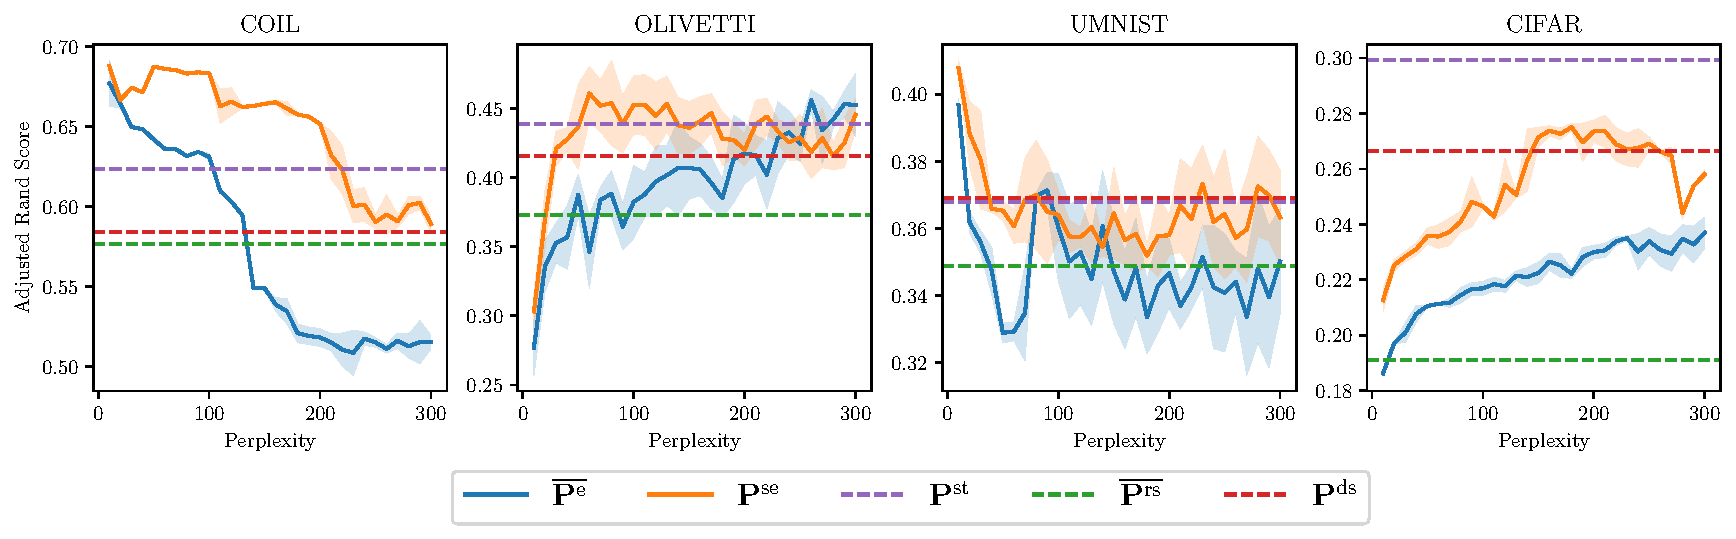
\includegraphics[width=\columnwidth]{figures/SNEkhorn/spectral_clustering_sensitivity.pdf}}
    \caption{ARI spectral clustering score as a function of the perplexity parameter for image datasets.}
    \label{fig:spectral_clustering_sensibility}
    \end{center}
    \vspace{-1.1cm}
\end{figure*}

\paragraph{Spectral Clustering.}
Building on the strong connections between spectral clustering mechanisms and t-SNE
\cite{van2022probabilistic,linderman2019clustering} we first consider spectral
clustering tasks to evaluate the affinity matrix $\Pb^{\mathrm{se}}$
\eqref{eq:sym_entropic_affinity} and compare it against
$\overline{\Pb^{\mathrm{e}}}$ \eqref{symmetrization_tsne}. We also consider two
versions of the Gaussian affinity with scalar bandwidth $\K = \exp(-\C/\nu)$:
the symmetrized row-stochastic $\overline{\Pb^{\mathrm{rs}}} =
\operatorname{Proj}^{\ell_2}_{\mathcal{S}}(\Pb^{\mathrm{rs}})$ where
$\Pb^{\mathrm{rs}}$ is $\K$ normalized by row and $\Pb^{\mathrm{ds}}$
\eqref{eq:plan_sym_sinkhorn}. We also consider the adaptive Self-Tuning
$\Pb^{\mathrm{st}}$ affinity from \cite{zelnik2004self} which relies on an
adaptive bandwidth corresponding to the distance from the $k$-th nearest
neighbor of each point. We use the spectral clustering implementation of
\texttt{scikit-learn} \cite{scikit-learn} with default parameters which uses the
unnormalized graph Laplacian. We measure the quality of clustering using the
Adjusted Rand Index (ARI). Looking at both \cref{table_spectral_microaray} and
\cref{fig:spectral_clustering_sensibility}, one can notice that, in general,
symmetric entropic affinities yield better results than usual entropic
affinities with significant improvements in some datasets (\eg throat microarray
and SNAREseq). Overall $\Pb^{\mathrm{se}}$ outperforms all the other affinities
in $8$ out of $12$ datasets. This shows that the adaptivity of EAs is crucial.
\cref{fig:spectral_clustering_sensibility} also shows that this
superiority is verified for the whole range of perplexities. This can be
attributed to the fact that symmetric entropic affinities combine the advantages
of doubly stochastic normalization in terms of clustering and of EAs in terms of
adaptivity. In the next experiment, we show that these advantages translate into
better clustering and neighborhood retrieval at the embedding level when running
SNEkhorn.

\begin{wrapfigure}[12]{R}{0.5\textwidth}
    \centerline{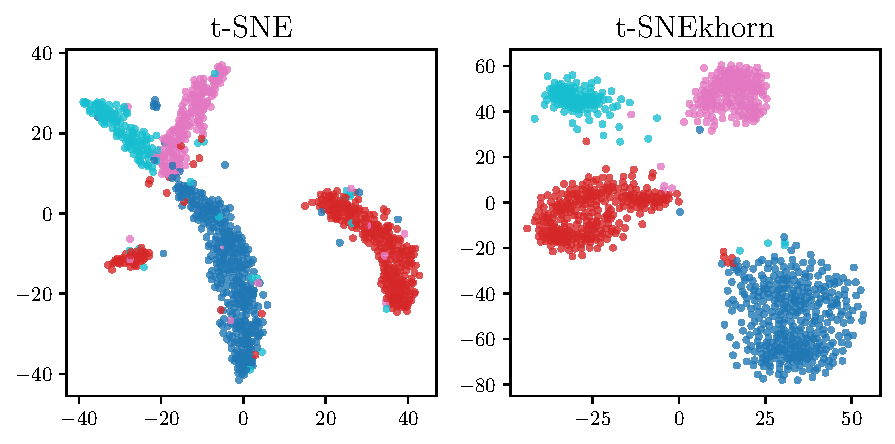
\includegraphics[width=\linewidth]{figures/SNEkhorn/fig_sc.pdf}}
    \captionof{figure}{SNAREseq embeddings produced by t-SNE and t-SNEkhorn with $\xi=50$.}
    \label{fig:sc}
\end{wrapfigure}

\paragraph{Dimension Reduction.}
To guarantee a fair comparison, we implemented not only SNEkhorn, but also t-SNE and UMAP in \texttt{PyTorch} \cite{paszke2017automatic}. 
% Note that UMAP also relies on adaptive affinities but sets the degree of each node (related to the hyperparameter \texttt{n\textunderscore neighbors} which plays a similar role to the perplexity) rather than the entropy.
% Our code is made available with this submission. 
All models were optimized using \texttt{ADAM} \cite{kingma2014adam} with default parameters and the same stopping criterion: the algorithm stops whenever the relative variation of the loss becomes smaller than $10^{-5}$. For each run, we draw independent $\mathcal{N}(0,1)$ coordinates and use this same matrix to initialize all the methods that we wish to compare. To evaluate the embeddings' quality, we make use of the silhouette \cite{rousseeuw1987silhouettes} and trustworthiness \cite{venna2001neighborhood} scores from \texttt{scikit-learn} \cite{scikit-learn} with default parameters.  While the former relies on class labels, the latter measures the agreement between the neighborhoods in input and output spaces, thus giving two complementary metrics to properly evaluate the embeddings. 
The results, presented in \cref{tab:DR_genomics_data}, demonstrate the notable superiority of t-SNEkhorn compared to the commonly used t-SNE and UMAP algorithms. Across the $16$ datasets examined, t-SNEkhorn almost consistently outperformed the others, achieving the highest silhouette score on $15$ datasets and the highest trustworthiness score on $12$ datasets. To visually assess the quality of the embeddings, we provide SNAREseq embeddings in \cref{fig:sc}. Notably, one can notice that the use of t-SNEkhorn results in improved class separation compared to t-SNE.
 
% \begin{table}[h]
% \caption{Silhouette scores ($\times 100$) for the datasets with most samples of the CuMiDa repository.}
% \label{tab:results_microarray}
% \vskip 0.1in
% \begin{center}
% \begin{small}
% \begin{sc}
% \begin{tabular}{lcccccc}
% \toprule
% Data set & t-SNE & UMAP & t-SNEkhor & t-SNE & UMAP & t-SNEkhornn \\
% \midrule
% Liver & 46.1$\pm$ 3.9 & 41.5$\pm$ 7.5& \textbf{58.5$\pm$ 1.0} & 46.1$\pm$ 3.9 & 41.5$\pm$ 7.5& \textbf{58.5$\pm$ 1.0} \\
% Breast & 24.0$\pm$ 5.6 & 21.8$\pm$ 9.6& \textbf{29.4$\pm$ 0.7} \\
% Leukemia & 14.6$\pm$ 5.1 & 9.1$\pm$ 7.4& \textbf{21.1$\pm$ 4.5} \\
% Colorectal & 61.1$\pm$ 2.4 & 58.5$\pm$ 7.7& \textbf{68.3$\pm$ 0.4} \\
% Liver \small{2} & 36.4$\pm$ 1.6 & 26.7$\pm$ 10& \textbf{45.8$\pm$ 0.9} \\
% Breast \small{2} & 26.5$\pm$ 3.2 & \textbf{32.2$\pm$ 2.7} & 30.7$\pm$ 3.8 \\
% Renal & 39.9$\pm$ 1.4 & \textbf{43.2$\pm$ 1.5} & 42.8$\pm$ 0.4 \\
% Brain & 11.1$\pm$ 5.3 & 7.6$\pm$ 7.2 & \textbf{16.3$\pm$ 4.3} \\
% \bottomrule
% \end{tabular}
% \end{sc}
% \end{small}
% \end{center}
% \vskip -0.1in
% \end{table}

\begin{table*}\centering
\caption{Scores for the UMAP, t-SNE and t-SNEkhorn embeddings.}
\vskip 0.1in
\begin{small}
\begin{tabular}{@{\hskip 0.1in}l@{\hskip 0.1in}c@{\hskip 0.1in}c@{\hskip 0.1in}c@{\hskip 0.1in}c@{\hskip 0.1in}c@{\hskip 0.1in}c@{\hskip 0.1in}c@{\hskip 0.1in}c@{\hskip 0.1in}}
    \toprule[1.5pt]
& \multicolumn{3}{c}{Silhouette ($\times 100$)} & & \multicolumn{3}{c}{Trustworthiness ($\times 100$)} \\
\cmidrule{2-4} \cmidrule{6-8}
& UMAP & t-SNE & t-SNEkhorn && UMAP & t-SNE & t-SNEkhorn \\ \midrule
COIL & $20.4\pm3.3$ & $30.7\pm6.9$ & $\mathbf{52.3\pm1.1}$ && $99.6\pm0.1$ & $99.6\pm0.1$ & $\mathbf{99.9\pm0.1}$ \\ 
OLIVETTI & $6.4\pm4.2$ & $4.5\pm3.1$ & $\mathbf{15.7\pm2.2}$ && $96.5\pm1.3$ & $96.2\pm0.6$ & $\mathbf{98.0\pm0.4}$ \\
UMNIST & $-1.4\pm2.7$ & $-0.2\pm1.5$ & $\mathbf{25.4\pm4.9}$ && $93.0\pm0.4$ & $99.6\pm0.2$ & $\mathbf{99.8\pm0.1}$ \\
CIFAR & $13.6\pm2.4$ & $18.3\pm0.8$ & $\mathbf{31.5\pm1.3}$ && $90.2\pm0.8$ & $90.1\pm0.4$ & $\mathbf{92.4\pm0.3}$ \\ \midrule[0.2pt]
Liver \tiny{(14520)} & $49.7\pm1.3$ & $50.9\pm0.7$ & $\mathbf{61.1\pm0.3}$ && $89.2\pm0.7$ & $90.4\pm0.4$ & $\mathbf{92.3\pm0.3}$ \\
Breast \tiny{(70947)} & $28.6\pm0.8$ & $29.0\pm0.2$ & $\mathbf{31.2\pm0.2}$ && $90.9\pm0.5$ & $91.3\pm0.3$ & $\mathbf{93.2\pm0.4}$ \\
Leukemia \tiny{(28497)} & $22.3\pm0.7$ & $20.6\pm0.7$ & $\mathbf{26.2\pm2.3}$ && $90.4\pm1.1$ & $92.3\pm0.8$ & $\mathbf{94.3\pm0.5}$ \\
Colorectal \tiny{(44076)} & $67.6\pm2.2$ & $69.5\pm0.5$ & $\mathbf{74.8\pm0.4}$ && $93.2\pm0.7$ & $93.7\pm0.5$ & $\mathbf{94.3\pm0.6}$ \\
Liver \tiny{(76427)} & $39.4\pm4.3$ & $38.3\pm0.9$ & $\mathbf{51.2\pm2.5}$ && $85.9\pm0.4$ & $89.4\pm1.0$ & $\mathbf{92.0\pm1.0}$ \\
Breast \tiny{(45827)} & $35.4\pm3.3$ & $39.5\pm1.9$ & $\mathbf{44.4\pm0.5}$ && $93.2\pm0.4$ & $94.3\pm0.2$ & $\mathbf{94.7\pm0.3}$ \\
Colorectal \tiny{(21510)} & $38.0\pm1.3$ & $\mathbf{42.3\pm0.6}$ & $35.1\pm2.1$ && $85.6\pm0.7$ & $\mathbf{88.3\pm0.9}$ & $88.2\pm0.7$ \\
Renal \tiny{(53757)} & $44.4\pm1.5$ & $45.9\pm0.3$ & $\mathbf{47.8\pm0.1}$ && $93.9\pm0.2$ & $\mathbf{94.6\pm0.2}$ & $94.0\pm0.2$ \\ 
Prostate \tiny{(6919)} & $5.4\pm2.7$ & $8.1\pm0.2$ & $\mathbf{9.1\pm0.1}$ && $77.6\pm1.8$ & $\mathbf{80.6\pm0.2}$ & $73.1\pm0.5$ \\ 
Throat \tiny{(42743)} & $26.7\pm2.4$ & $28.0\pm0.3$ & $\mathbf{32.3\pm0.1}$ && $\mathbf{91.5\pm1.3}$ & $88.6\pm0.8$ & $86.8\pm1.0$ \\ \midrule[0.2pt]
scGEM & $26.9\pm3.7$ & $33.0\pm1.1$ & $\mathbf{39.3\pm0.7}$ && $95.0\pm1.3$ & $96.2\pm0.6$ & $\mathbf{96.8\pm0.3}$ \\
SNAREseq & $6.8\pm6.0$ & $35.8\pm5.2$ & $\mathbf{67.9\pm1.2}$ && $93.1\pm2.8$ & $99.1\pm0.1$ & $\mathbf{99.2\pm0.1}$ \\
\bottomrule[1.5pt]
\label{tab:DR_genomics_data}
\end{tabular}
\end{small}
\vspace*{-0.5cm}
\end{table*}


% \begin{table*}\centering
%     \ra{1.3}
%     \caption{Scores for the SNE, \texttt{DOSNES} and SNEkhorn embeddings on the images datasets.}
%     \vskip 0.1in
%     \begin{small}
%     \begin{tabular}{@{}lccccccc@{}}\toprule
%     & \multicolumn{3}{c}{Silhouette score ($\times 100$)} & & \multicolumn{3}{c}{Trustworthiness ($\times 100$)} \\
%     \cmidrule{2-4} \cmidrule{6-8}
%     & SNE & \texttt{DOSNES} & SNEkhorn && SNE & \texttt{DOSNES} & SNEkhorn \\ \midrule
%     COIL & 32.5$\pm$1.5 & & \textbf{37.6$\pm$3.2} && 98.1$\pm$0.4 & & \textbf{98.4$\pm$0.1} \\
%     OLIVETTI & 4.5$\pm$3.1 & & \textbf{15.7$\pm$2.2} && 96.2$\pm$0.6 & & \textbf{98.0$\pm$0.4} \\
%     UMNIST & & & && & & \\
%     CIFAR & & & && & & \\
%     \bottomrule
%     \label{tab:DR_genomics_data}
%     \end{tabular}
%     \end{small}
% \end{table*}
    